\documentclass[
12pt,
a4paper,
oneside,
headinclude,
footinclude]{article}

\usepackage[table,xcdraw,svgnames, dvipsnames]{xcolor}
\usepackage[capposition=bottom]{floatrow}
\usepackage[colorlinks]{hyperref} % to add hyperlinks
\usepackage{enumitem}
\usepackage{booktabs}
\usepackage{tabularx}
\usepackage{csquotes}
\usepackage{amsmath} % For the big bracket
\usepackage[export]{adjustbox}[2011/08/13]
\usepackage{array}
\usepackage{url}
\usepackage{graphicx} % to insert images
\usepackage{titlepic} % to insert image on front page
\usepackage{geometry} % to define margin
\usepackage{listings} % to add code
\usepackage{caption}
\usepackage[T1]{fontenc} % Use 8-bit encoding that has 256 glyphs
\usepackage[utf8]{inputenc} % Required for including letters with accents
\usepackage{color}
\usepackage{subcaption}
\usepackage[nochapters, dottedtoc]{classicthesis}
\usepackage{listings} % For Python code

\usepackage[ruled]{algorithm2e} % For pseudo-code

\usepackage{mathpazo}

\usepackage{lipsum} % For testing
\usepackage{color}

\usepackage{etoolbox}

\usepackage{tikz} % For trees plot
\usepackage{tikz-dependency} % For dependency graphs

\usepackage{bm} % For bold math

\usepackage{setspace}
\usepackage{minted}

% For tables
\usepackage{amssymb}

\definecolor{dkgreen}{rgb}{0,0.6,0}
\definecolor{gray}{rgb}{0.5,0.5,0.5}
\definecolor{mauve}{rgb}{0.58,0,0.82}

% ==== Define python syntax ====
\definecolor{Code}{rgb}{0,0,0}
\definecolor{Decorators}{rgb}{0.5,0.5,0.5}
\definecolor{Numbers}{rgb}{0.5,0,0}
\definecolor{MatchingBrackets}{rgb}{0.25,0.5,0.5}
\definecolor{Keywords}{rgb}{0,0,1}
\definecolor{self}{rgb}{0,0,0}
\definecolor{Strings}{rgb}{0,0.63,0}
\definecolor{Comments}{rgb}{0,0.63,1}
\definecolor{Backquotes}{rgb}{0,0,0}
\definecolor{Classname}{rgb}{0,0,0}
\definecolor{FunctionName}{rgb}{0,0,0}
\definecolor{Operators}{rgb}{0,0,0}
\definecolor{Background}{rgb}{0.98,0.98,0.98}
\lstdefinelanguage{Python}{
    numbers=left,
    numberstyle=\footnotesize,
    numbersep=1em,
    xleftmargin=1em,
    framextopmargin=2em,
    framexbottommargin=2em,
    showspaces=false,
    showtabs=false,
    showstringspaces=false,
    frame=l,
    tabsize=4,
    % Basic
    basicstyle=\ttfamily\small\setstretch{1},
    backgroundcolor=\color{Background},
    % Comments
    commentstyle=\color{Comments}\slshape,
    % Strings
    stringstyle=\color{Strings},
    morecomment=[s][\color{Strings}]{"""}{"""},
    morecomment=[s][\color{Strings}]{'''}{'''},
    % keywords
    morekeywords={import,from,class,def,for,while,if,is,in,elif,else,not,and,or,print,break,continue,return,True,False,None,access,as,,del,except,exec,finally,global,import,lambda,pass,print,raise,try,assert},
    keywordstyle={\color{Keywords}\bfseries},
    % additional keywords
    morekeywords={[2]@invariant,pylab,numpy,np,scipy},
    keywordstyle={[2]\color{Decorators}\slshape},
    emph={self},
    emphstyle={\color{self}\slshape},
    %
}


\lstset{language=Python}

\definecolor{webbrown}{rgb}{.6,0,0}

\usepackage{titlesec} % to customize titles
\titleformat{\chapter}{\normalfont\huge}{\textbf{\thechapter.}}{20pt}{\huge\textbf}[\vspace{2ex}\titlerule] % to customize chapter title aspect
\titleformat{\section} % to customize section titles
{\fontsize{14}{15}\bfseries}{\thesection}{1em}{}

\titlespacing*{\chapter}{0pt}{-50pt}{20pt} % to customize chapter title space

\graphicspath{ {../Figures/} } % images folder
\parindent0pt \parskip10pt % make block paragraphs
\geometry{verbose,tmargin=3cm,bmargin=3cm,lmargin=3cm,rmargin=3cm,headheight=3cm,headsep=3cm,footskip=1cm} % define margin
\hyphenation{Fortran hy-phen-ation}

\AtBeginDocument{%
    \hypersetup{
        colorlinks=true, breaklinks=true, bookmarks=true,
        urlcolor=webbrown, citecolor=Black, linkcolor=Black% Link colors
}}

\pagestyle{plain}
\title{\textbf{NLP Assignment 2: \\ Dependency Relations \&\\
        Transition-based Parser}}
\author{{Alberto Parravicini}}
\date{}	% default \today

% =============================================== BEGIN


\begin{document}
    \maketitle
    \pagenumbering{roman}
    \setcounter{page}{1}
    
    \section{Introduction}
    
    Among the many formalisms to represent the structure of a sentence, \textbf{Dependency grammars} provide a flexible and intuitive way to describe how words relate to each other. \\
    \textit{Dependency grammars} describe the dependencies between words, e.g. to which \textit{noun} a certain \textit{adjective} refers.\\
    Each sentence is represented as a directed tree in which each word $\{w_1,\ w_2,\ \ldots,\ w_n\}$ is a vertex of the tree, and there exists an arc from word $w_i$ to word $w_j$ if and only if word $w_j$ depends on word $w_i$. In this relation, $w_i$ is referred as \textbf{head}, while $w_j$ is the \textbf{dependent}.\\
    By convention, we say that the main verb of a sentence is the \textbf{root}, and has no incoming arcs.
    
    As a simple example, in the sentence \textit{you sing} the verb \textit{sing} will have an arc to the pronoun \textit{you}, as the latter is a subject of the former.\\
    Furthermore, arcs can be labelled, in order to explicitly say what type of dependency, or \textbf{grammatical function}, occurs between two words: in the previous example, the arc would be labelled as \textbf{nsubj}, as \textit{you} is the subject of \textit{sing}.
    The full set of dependency relations can be found \href{http://universaldependencies.org/u/dep/index.html}{here}.
    
    This model, by definition, is purely \textit{descriptive}, i.e. it doesn't say how relations between words should be assigned. \\
    To do so, it will be necessary to build a \textbf{parser}, an algorithm which scans the sentence and assigns the appropriate relations between each pair of words.\\
    The construction of a parser will be the focus of \textit{section 2} onwards; first, however, we can look at some examples of dependency relations, to get a better understanding of how \textit{dependency grammars} work.
    
    
    \section{Annotation of sentences}
    
    Given a small set of sentences, we can annotate them as described in the \textbf{\href{http://universaldependencies.org/format.html}{CoNNL-U}} format.
    For each word, we denote its \textit{lemma}, its \textit{part-of-speech} (\textbf{POS}, according to the \href{http://universaldependencies.org/u/pos/index.html}{universal part-of-speech tags}), its \textit{head} and \textit{dependency relation}, as defined above. The \textbf{CoNNL-U} format contains other fields, but for our purpose they can be omitted.\\
    
    The sentences that we consider are, in order:
    
    \begin{enumerate}
        \item I gave an apple to the teacher
        \item Mary missed her train to work
        \item John gave the teacher a very heavy book 
        \item The sun shines 
        \item This is the dog that chased the cat 
        \item I saw the doctor this morning who is treating me 
        \item This is the cat that the dog chased 
        \item John is eager to please  
    \end{enumerate} 

    The full annotaion of each sentence if given in the file \textbf{annotation.txt}.
    For the first sentence (\textit{I gave an apple to the teacher}) are provided a \textit{dependency tree} and a \textit{dependency diagram}, which also shows the type of grammatical relation between the words.
       
    
    \begin{center}
        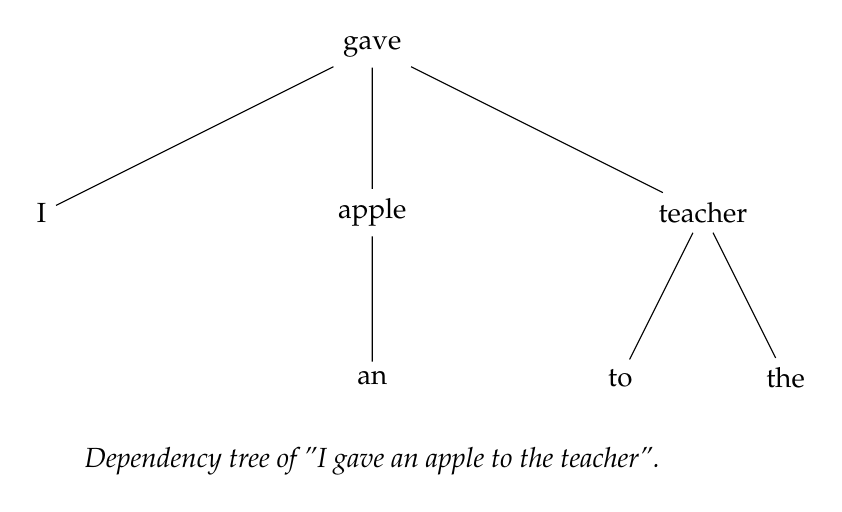
\begin{tikzpicture}[scale=1.4]
        \node (is-root) {gave}
        [sibling distance=3cm]
        child { node {I} }
        child {
            node {apple}
            [sibling distance=1.5cm]
            child { node {an} }
        }
        child { node {teacher}
            [sibling distance=1.5cm]
            child { node {to} }
            child { node {the} }
        };
        \path (is-root) +(0,-2.5\tikzleveldistance)
        node {\textit{Dependency tree of "I gave an apple to the teacher".}};
        \end{tikzpicture}
    \end{center}
   
    \begin{center}
        \scalebox{1.1} {
        \begin{dependency}[theme = simple]
            \begin{deptext}[column sep=1em, row sep=0.5ex]
                I \& gave \& an \& apple \& to \& the \& teacher \\
                PRON \& VERB \& DET \& NOUN \& ADP \& DET \& NOUN \\
            \end{deptext}
            \deproot{2}{ROOT}
            \depedge{2}{1}{NSUBJ}
            %\depedge[edge start x offset=-6pt]{2}{5}{ATT}
            \depedge{2}{4}{OBJ}
            \depedge[edge start x offset=-1pt]{4}{3}{DET}
            \depedge{2}{7}{OBL}
            \depedge{7}{5}{CASE}
            \depedge[edge start x offset=-5pt]{7}{6}{DET}
            %\depedge[arc angle=50]{7}{6}{ATT}
        \end{dependency}
        }
    \end{center}

    The structure of the sentence is rather simple, and can be represented as \textbf{subject} $+$ \textbf{verb} $+$ \textbf{object} $+$ \textbf{indirect object}; note that the indirect object is defined \textit{oblique}, and the \textbf{to} apposition is called \textit{case}.
    
    As for the other sentences, we can make the following observations:
    
    \begin{itemize}
        \item In some sentences, certain words could have more than one \textit{part-of-speech} tag. However, in most cases only one tag is grammatically correct, given the context.
        \item As an example, in the second sentence the word \textit{work} can be seen as a noun or as a verb, but given the context only the former interpretation is valid. The same applies to sentence 4 (\textit{shines} can be a - rather unusual - noun). 
        \item \textbf{That} can be either a \textit{determinant} (as in \textit{that book}) or a \textit{subordinating conjunction}, as in sentence 5.
        \item \textit{This morning} can be seen as a \textit{determinant} followed by a \textit{noun}, or as a single \textit{temporal adverb}, composed by 2 words. In this case, both options are grammatically correct.
        \item Sentence 6 could be seen as \textit{non-projective}: specifically, if we say that \textit{treating} depends from \textit{doctor}, then the arc that joins the 2 words will be \textit{non-projective}, as there is no path from \textit{doctor} to \textit{this morning}.\\
        However, it is also possible to interpret the sentence in a way that \textit{treating} depends from the main verb \textit{saw}, and in this case the sentence would be projective.\\
        In this case, the non-projectivity arises from the fact that \textit{this morning} can be placed rather freely in a sentence: it could be at the start, in the middle, or at the end, and in every case the sentence would be grammatically correct.
    \end{itemize}

    
    \section{Implementation of the parser}
    
    In order to assign correct dependency relations to each word in the sentence, we have to build a parser: in our case, the parser will take the form of a greedy \textit{shift-reduce} algorithm.\\
    At each step, the algorithm will decide which action to take: whether to read a word from the input buffer, or to assign a \textit{dependency relation}. For simplicity, we consider only \textbf{left} arcs, \textbf{right} arcs, and \textbf{shifts}. No other dependency relation is specified.
    
    Words that are read from the input buffer are placed in a stack: then, the algorithm will decide which action to take, based on the content of the stack and of the input buffer. If a dependency relation is added, a word is removed from the stack. The stack is initialized with a special element denoted as \textbf{\_\_ROOT\_\_}.
    
    Now, there are two issues to discuss.
    
    First, when should a \textit{left} or \textit{right} action be taken?\\
    When a \textit{left} arc is assigned, the dependent word is removed from the stack. As such, we can assign left arcs without many complications: the only borderline case is when the root is the second element in the stack.\\
    In that case, it is forbidden to assign a \textit{left} arc, as it would imply that the root is dependent from some other word!\\
    Right actions are more complex to handle: the assignment of a right arc will lead to the removal of te \textbf{head}, and as a consequence we must be sure that all the words dependent on that head have already been marked with a \textit{left} arc; otherwise it will be impossible to flag them correctly, as their head has been removed.\\
    In our algorithm, the assignment of right arcs is problematic as we can be sure that a word has no other dependents only after reading the entire sentence. Without being able to do so, we must be able to predict efficiently if a word will have some other dependent further down the sentence.
    
    The second issue is related to how the action to be made is chosen. Ideally, we would have an omniscient oracle that always spits out the right action to be performed.\\
    More realistically, our oracle will have to predict the best action given the current state of the parser, i.e. the stack and the input buffer. \\
    This prediction can be done by extracting features from the state, such as the \textit{part-of-speech} tags of the words in the stack and in the input buffer.
    
    The features can on paper be computed by the parser itself, and fed as input to the oracle. However, a more flexible approach consists in passing the state of the parser to the oracle, and leave the feature construction to the oracle itself. \\
    This approach has the advantage of isolating completely the oracle from the parser: it is easily possible to use different kinds of oracles, without having to modify at all the parser algorithm. 
    
    In the proposed implementation, we initially experiment with a vary basic oracle that will provide random actions (given some reasonable constraints, such as not shifting if the buffer is empty), then move to a \textbf{rule-based} oracle.
    
    The rule based oracle is built by inspecting the structure of the first 4 sentences given before. To provide more versatility, the oracle will look at the \textit{part-of-speech} tags of the words, not at the words themselves.\\
    Moreover, the oracle will look at the first and second words on the stack and in the input buffer. \\
    Rules are provided as \textit{if-else} statements, and as such there is no reason no explicitly build 2-words features (i.e. features build by using two words), as we can simply combine the single word features inside the \textit{if-else} statements.
    
    For the explanation of the meaning and the role of each single rule, please refer to the comments in the code. Still, it is possible to make some more general considerations regarding the structure of the rules.
    
    These rules are quite similar to the ones used by \textbf{Classification rules} algorithms, and the same line of thoughts can be applied to the construction of the oracle's rules.
    
    \begin{itemize}
        \item A general idea, is that the first rules to be considered, i.e. the ones at the top, should be the most restrictive ones, and match the most specific cases. As an example, it is considered the rules that matches the pattern \textbf{"verb"} $+$ \textbf{"det"} $+$ \textbf{"adv/adj"} $+$ \textbf{"adv/adj"}, which is usually followed by a nominal to which the last two elements refer (as in sentence 3); as such, it is appropriate to shift. 
        \item To cover situations that are not matched by any rule, it is important to have a default rule: in our case, a random action will work, provided that no constraint is violated (in that case, the action is changed appropriately).
        \item In general, it would be preferrable to have non-overlapping rules: overlaps occur when a single input is matched by more than one rule: in this case, the first rule to appear is the one that will be used. \\
        Measuring if rules overlap is quite difficult, but as a rule of thumb having restricting rules at the top should avoid unwanted behaviours.
    \end{itemize}
    
    On a side note, the features generated by the \textbf{rule-based} oracle have been saved to a file (\textbf{feattemp.txt}), along with the action that correspond to each feature vector. This dataset has been used to train a simple decision tree, to see if it would be able to reconstruct, or even improve, the results of the rule-based oracle.\\
    However, the results are very poor, as the tree is unable to predict \textit{right arcs}, as seen by the drawing of the tree structure (in the file \textit{tree.pdf}).
    
    \subsection{Execution traces}
    Below are reported the execution traces of the parsing of the first 4 sentences.

    \begin{center}
        \begin{table}[H]   
            \hspace*{-2.0cm}
            \begin{tabular}{l p{5cm} p{5cm} l l} % creating eight columns
                \hline
                \hline 
                \\[-1.5ex]
                \textcolor{BrickRed}{Step} & \textcolor{BrickRed}{Stack} & \textcolor{BrickRed}{Buffer} & \textcolor{BrickRed}{Action} & \textcolor{BrickRed}{Output}\\ [0.5ex]
                \hline % inserts single-line
                \\[-1.5ex]
                0 & [\_\_ROOT\_\_] & [I, gave, an, apple, to, the, teacher] & SHIFT & \\ 
                1 & [\_\_ROOT\_\_, I] & [gave, an, apple, to, the, teacher] & SHIFT & \\ 
                2 & [\_\_ROOT\_\_, I, gave] & [an, apple, to, the, teacher] & LEFT & ( I $\rightarrow$ gave )\\ 
                3 & [\_\_ROOT\_\_, gave] & [an, apple, to, the, teacher] & SHIFT & \\ 
                4 & [\_\_ROOT\_\_, gave, an] & [apple, to, the, teacher] & SHIFT & \\ 
                5 & [\_\_ROOT\_\_, gave, an, apple] & [to, the, teacher] & LEFT & ( an $\leftarrow$ apple )\\ 
                6 & [\_\_ROOT\_\_, gave, apple] & [to, the, teacher] & RIGHT & ( gave $\rightarrow$ apple )\\ 
                7 & [\_\_ROOT\_\_, gave] & [to, the, teacher] & SHIFT & \\ 
                8 & [\_\_ROOT\_\_, gave, to] & [the, teacher] & SHIFT & \\ 
                9 & [\_\_ROOT\_\_, gave, to, the] & [teacher] & SHIFT & \\ 
                10 & [\_\_ROOT\_\_, gave, to, the, teacher] & [] & LEFT & ( the $\leftarrow$ teacher )\\ 
                11 & [\_\_ROOT\_\_, gave, to, teacher] & [] & LEFT & ( to $\leftarrow$ teacher )\\ 
                12 & [\_\_ROOT\_\_, gave, teacher] & [] & RIGHT & ( gave $\rightarrow$ teacher )\\ 
                13 & [\_\_ROOT\_\_, gave] & [] & RIGHT & ( \_\_ROOT\_\_ $\rightarrow$ gave )\\ 
                14 & [\_\_ROOT\_\_] & [] & DONE &                 
                \\[1ex] % [1ex] adds vertical space
                \hline % inserts single-line
            \end{tabular}
            \caption{\label{tab:trace-1}Execution trace for \textit{I gave an apple to the teacher}.}
        \end{table} 
    \end{center}

    \begin{center}
    \begin{table}[H]   
        \hspace*{-2.0cm}
        \begin{tabular}{l p{5cm} p{5cm} l l} % creating eight columns
            \hline
            \hline 
            \\[-1.5ex]
            \textcolor{BrickRed}{Step} & \textcolor{BrickRed}{Stack} & \textcolor{BrickRed}{Buffer} & \textcolor{BrickRed}{Action} & \textcolor{BrickRed}{Output}\\ [0.5ex]
            \hline % inserts single-line
            \\[-1.5ex]
            0 & [\_\_ROOT\_\_] & [Mary, missed, her, train, to, work] & SHIFT & \\ 
            1 & [\_\_ROOT\_\_, Mary] & [missed, her, train, to, work] & SHIFT & \\ 
            2 & [\_\_ROOT\_\_, Mary, missed] & [her, train, to, work] & LEFT & ( Mary $\leftarrow$ missed )\\ 
            3 & [\_\_ROOT\_\_, missed] & [her, train, to, work] & SHIFT & \\ 
            4 & [\_\_ROOT\_\_, missed, her] & [train, to, work] & SHIFT & \\ 
            5 & [\_\_ROOT\_\_, missed, her, train] & [to, work] & LEFT & ( her $\leftarrow$ train )\\ 
            6 & [\_\_ROOT\_\_, missed, train] & [to, work] & RIGHT & ( missed $\rightarrow$ train )\\ 
            7 & [\_\_ROOT\_\_, missed] & [to, work] & SHIFT & \\ 
            8 & [\_\_ROOT\_\_, missed, to] & [work] & SHIFT & \\ 
            9 & [\_\_ROOT\_\_, missed, to, work] & [] & LEFT & ( to $\leftarrow$ work )\\ 
            10 & [\_\_ROOT\_\_, missed, work] & [] & RIGHT & ( missed $\rightarrow$ work )\\ 
            11 & [\_\_ROOT\_\_, missed] & [] & RIGHT & ( \_\_ROOT\_\_ $\rightarrow$ missed )\\ 
            12 & [\_\_ROOT\_\_] & [] & DONE &             
            \\[1ex] % [1ex] adds vertical space
            \hline % inserts single-line
        \end{tabular}
        \caption{\label{tab:trace-2}Execution trace for \textit{Mary missed her train to work}.}
    \end{table} 
    \end{center}


    \begin{center}
    \begin{table}[H]   
        \hspace*{-2.0cm}
        \begin{tabular}{l p{5cm} p{5cm} l l} % creating eight columns
            \hline
            \hline 
            \\[-1.5ex]
            \textcolor{BrickRed}{Step} & \textcolor{BrickRed}{Stack} & \textcolor{BrickRed}{Buffer} & \textcolor{BrickRed}{Action} & \textcolor{BrickRed}{Output}\\ [0.5ex]
            \hline % inserts single-line
            \\[-1.5ex]
            0 & [\_\_ROOT\_\_] & [John, gave, the, teacher, a, very, heavy, book] & SHIFT & \\ 
            1 & [\_\_ROOT\_\_, John] & [gave, the, teacher, a, very, heavy, book] & SHIFT & \\ 
            2 & [\_\_ROOT\_\_, John, gave] & [the, teacher, a, very, heavy, book] & LEFT & ( John $\leftarrow$ gave )\\ 
            3 & [\_\_ROOT\_\_, gave] & [the, teacher, a, very, heavy, book] & SHIFT & \\ 
            4 & [\_\_ROOT\_\_, gave, the] & [teacher, a, very, heavy, book] & SHIFT & \\ 
            5 & [\_\_ROOT\_\_, gave, the, teacher] & [a, very, heavy, book] & LEFT & ( the $\leftarrow$ teacher )\\ 
            6 & [\_\_ROOT\_\_, gave, teacher] & [a, very, heavy, book] & RIGHT & ( gave $\rightarrow$ teacher )\\ 
            7 & [\_\_ROOT\_\_, gave] & [a, very, heavy, book] & SHIFT & \\ 
            8 & [\_\_ROOT\_\_, gave, a] & [very, heavy, book] & SHIFT & \\ 
            9 & [\_\_ROOT\_\_, gave, a, very] & [heavy, book] & SHIFT & \\ 
            10 & [\_\_ROOT\_\_, gave, a, very, heavy] & [book] & LEFT & ( very $\leftarrow$ heavy )\\ 
            11 & [\_\_ROOT\_\_, gave, a, heavy] & [book] & SHIFT & \\ 
            12 & [\_\_ROOT\_\_, gave, a, heavy, book] & [] & LEFT & ( heavy $\leftarrow$ book )\\ 
            13 & [\_\_ROOT\_\_, gave, a, book] & [] & LEFT & ( a $\leftarrow$ book )\\ 
            14 & [\_\_ROOT\_\_, gave, book] & [] & RIGHT & ( gave $\rightarrow$ book )\\ 
            15 & [\_\_ROOT\_\_, gave] & [] & RIGHT & ( \_\_ROOT\_\_ $\rightarrow$ gave )\\ 
            16 & [\_\_ROOT\_\_] & [] & DONE &           
            \\[1ex] % [1ex] adds vertical space
            \hline % inserts single-line
        \end{tabular}
        \caption{\label{tab:trace-2}Execution trace for \textit{John gave the teacher a very heavy book}.}
    \end{table} 
    \end{center}
    
    
    \begin{center}
    \begin{table}[H]   
        \hspace*{-2.0cm}
        \begin{tabular}{l p{5cm} p{5cm} l l} % creating eight columns
            \hline
            \hline 
            \\[-1.5ex]
            \textcolor{BrickRed}{Step} & \textcolor{BrickRed}{Stack} & \textcolor{BrickRed}{Buffer} & \textcolor{BrickRed}{Action} & \textcolor{BrickRed}{Output}\\ [0.5ex]
            \hline % inserts single-line
            \\[-1.5ex]
            0 & [\_\_ROOT\_\_] & [The, sun, shines] & SHIFT & \\ 
            1 & [\_\_ROOT\_\_, The] & [sun, shines] & SHIFT & \\ 
            2 & [\_\_ROOT\_\_, The, sun] & [shines] & LEFT & ( The $\leftarrow$ sun )\\ 
            3 & [\_\_ROOT\_\_, sun] & [shines] & SHIFT & \\ 
            4 & [\_\_ROOT\_\_, sun, shines] & [] & LEFT & ( sun $\leftarrow$ shines )\\ 
            5 & [\_\_ROOT\_\_, shines] & [] & RIGHT & ( \_\_ROOT\_\_ $\rightarrow$ shines )\\ 
            6 & [\_\_ROOT\_\_] & [] & DONE &     
            \\[1ex] % [1ex] adds vertical space
            \hline % inserts single-line
        \end{tabular}
        \caption{\label{tab:trace-2}Execution trace for \textit{The sun shines}.}
    \end{table} 
    \end{center}
    
    \section{Parser Evaluation}
    After parsing the sentences, we can inspect what is the accuracy of our parser. We can notice how the parser is able to predict the dependency relations with $100\%$ accuracy, and (obviously) values of $100\%$ also in terms of precision and recall relatively to the 3 actions. \\
    With such a small test set it is hard to say if some rules were over-specific, or if the results are explained by the rather simple structure of the 4 sentences that were tested.
    
    To get some further insight of the performances of the model, we could test it against the other 4 sentences that we were given.\\
    It should be immediately pointed out that the results will be mediocre at best, as our \textbf{rule-based} oracle doesn't keep into account some of the \textit{part-of-speech} tags that appear in the other sentences. \\
    Still, this test could shed some light on the weaknesses of the model we built.
    
    The input and the output of this test are saved as \textbf{input\_test.txt} and \textbf{output\_test.txt}.
    
    On these test sequences, we can note the following:
    
    \begin{itemize}
        \item The oracle is unable to identify a \textit{determiner} as subject of the fifth sentence. It will not be able to recognize the main verb as root of the sentence, so it will either read the entire input buffer and proceed to assign dependencies at random (or by recognizing some simple pattern, such as \textit{determiner} $+$ \textit{noun}), or it will pick the verb of a subordinate clause as main verb.
        \item In the fifth and sixth sentences the oracle is unable to handle the subordinate clauses. Specifically, it can't handle the fact that the verb of the subordinate is dependent on the main verb.
        \item The seventh sentence has similar problems as before: a determiner as subject, and a relative clause.
        \item In the sixth and in the eight sentences, the parser cannot recognize the role of the auxiliary verb. In the first case the oracle can still recognize the second part of the verb, but in the last sentence the auxiliary verb is used as copula, and the parser cannot identify the main verb of the sentence.
    \end{itemize}
    
    On the test sentences, we can measure an overall accuracy of $\frac{15}{31} = 0.48$, including the root arcs.
    Moreover, we have an accuracy of $\frac{8}{15} = 0.53$ for the left arcs and of $\frac{5}{12} = 0.41$ for the right arcs (root arcs are not included in this case).\\
    The data seems to partially confirm the intuition that right arcs are more difficult to predict, even tough the sample size at our disposal is too small to draw any definitive conclusion.    
\end{document}